\documentclass{standalone}
\usepackage{tikz}
\usetikzlibrary{patterns, positioning}
\usepackage[sfdefault]{ClearSans} %% option 'sfdefault' activates Clear Sans as the default text font
\usepackage[T1]{fontenc}

\begin{document}
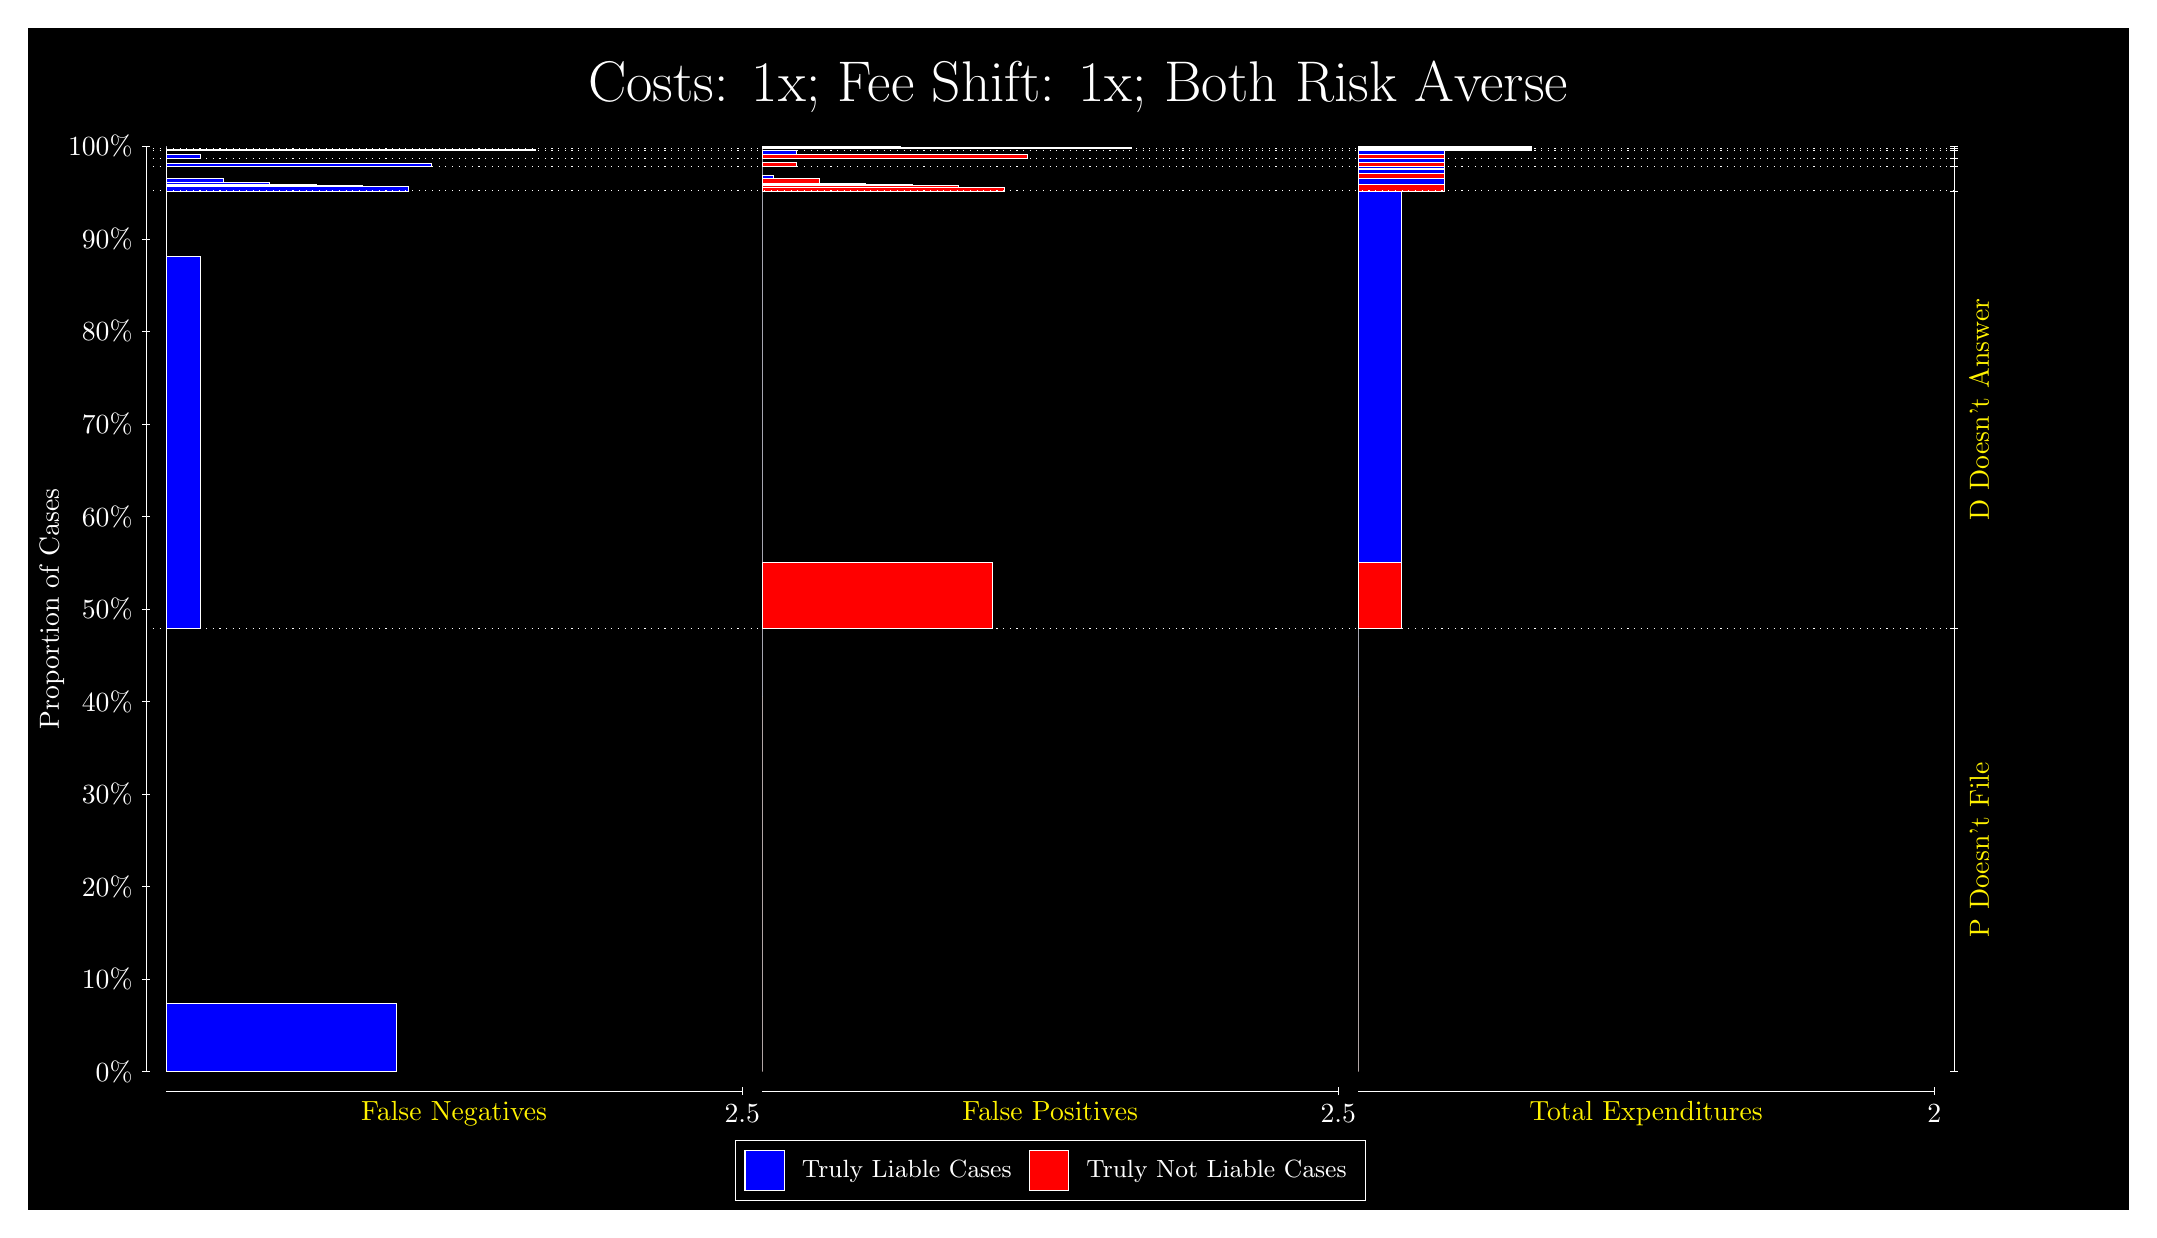
\begin{tikzpicture}
\draw[fill=black] (0,0) rectangle (26.667,15);
\draw[text=white] (0,13.5) rectangle (26.667,15) node[midway] {\huge Costs: 1x; Fee Shift: 1x; Both Risk Averse};
\draw[white, very thin] (1.5,1.75) -- (1.5,13.5);
\node[rotate=90, text=white, anchor=center] at (0.3, 7.625) {Proportion of Cases};
\draw[white, very thin] (1.45,1.75) -- (1.55,1.75);
\node[text=white, anchor=east] at (1.45, 1.75) {0\%};
\draw[white, very thin] (1.45,2.925) -- (1.55,2.925);
\node[text=white, anchor=east] at (1.45, 2.925) {10\%};
\draw[white, very thin] (1.45,4.1) -- (1.55,4.1);
\node[text=white, anchor=east] at (1.45, 4.1) {20\%};
\draw[white, very thin] (1.45,5.275) -- (1.55,5.275);
\node[text=white, anchor=east] at (1.45, 5.275) {30\%};
\draw[white, very thin] (1.45,6.45) -- (1.55,6.45);
\node[text=white, anchor=east] at (1.45, 6.45) {40\%};
\draw[white, very thin] (1.45,7.625) -- (1.55,7.625);
\node[text=white, anchor=east] at (1.45, 7.625) {50\%};
\draw[white, very thin] (1.45,8.8) -- (1.55,8.8);
\node[text=white, anchor=east] at (1.45, 8.8) {60\%};
\draw[white, very thin] (1.45,9.975) -- (1.55,9.975);
\node[text=white, anchor=east] at (1.45, 9.975) {70\%};
\draw[white, very thin] (1.45,11.15) -- (1.55,11.15);
\node[text=white, anchor=east] at (1.45, 11.15) {80\%};
\draw[white, very thin] (1.45,12.325) -- (1.55,12.325);
\node[text=white, anchor=east] at (1.45, 12.325) {90\%};
\draw[white, very thin] (1.45,13.5) -- (1.55,13.5);
\node[text=white, anchor=east] at (1.45, 13.5) {100\%};

\draw[white, very thin] (24.457,1.75) -- (24.457,13.5);
\draw[white, very thin] (24.407,1.75) -- (24.507,1.75);
\node[anchor=west] at (24.407, 1.75) {};
\draw[white, very thin] (24.407,7.3773) -- (24.507,7.3773);
\node[anchor=west] at (24.407, 7.3773) {};
\draw[white, very thin] (24.407,12.934) -- (24.507,12.934);
\node[anchor=west] at (24.407, 12.934) {};
\draw[white, very thin] (24.407,13.243) -- (24.507,13.243);
\node[anchor=west] at (24.407, 13.243) {};
\draw[white, very thin] (24.407,13.347) -- (24.507,13.347);
\node[anchor=west] at (24.407, 13.347) {};
\draw[white, very thin] (24.407,13.45) -- (24.507,13.45);
\node[anchor=west] at (24.407, 13.45) {};
\draw[white, very thin] (24.407,13.475) -- (24.507,13.475);
\node[anchor=west] at (24.407, 13.475) {};
\draw[white, very thin] (24.407,13.5) -- (24.507,13.5);
\node[anchor=west] at (24.407, 13.5) {};

\draw[white, very thin, fill=blue] (1.75,1.75) rectangle (4.6775,2.6195);
\draw[white, very thin, fill=red] (1.75,2.6195) rectangle (1.75,7.3773);
\draw[white, very thin, fill=blue] (1.75,7.3773) rectangle (2.1891,12.1);
\draw[white, very thin, fill=red] (1.75,12.1) rectangle (1.75,12.934);
\draw[white, very thin, fill=blue] (1.75,12.934) rectangle (4.8239,12.988);
\draw[white, very thin, fill=blue] (1.75,12.988) rectangle (4.2384,13.005);
\draw[white, very thin, fill=blue] (1.75,13.005) rectangle (3.9457,13.005);
\draw[white, very thin, fill=blue] (1.75,13.005) rectangle (3.6529,13.017);
\draw[white, very thin, fill=blue] (1.75,13.017) rectangle (3.3602,13.018);
\draw[white, very thin, fill=blue] (1.75,13.018) rectangle (3.0674,13.04);
\draw[white, very thin, fill=blue] (1.75,13.04) rectangle (2.4819,13.089);
\draw[white, very thin, fill=red] (1.75,13.089) rectangle (1.75,13.243);
\draw[white, very thin, fill=blue] (1.75,13.243) rectangle (5.1167,13.29);
\draw[white, very thin, fill=red] (1.75,13.29) rectangle (1.75,13.347);
\draw[white, very thin, fill=blue] (1.75,13.347) rectangle (2.1891,13.403);
\draw[white, very thin, fill=red] (1.75,13.403) rectangle (1.75,13.45);
\draw[white, very thin, fill=blue] (1.75,13.45) rectangle (6.4341,13.458);
\draw[white, very thin, fill=red] (1.75,13.458) rectangle (1.75,13.475);
\draw[white, very thin, fill=red] (1.75,13.475) rectangle (1.75,13.483);
\draw[white, very thin, fill=blue] (1.75,13.483) rectangle (1.75,13.5);
\draw[white, very thin, fill=red] (9.3189,1.75) rectangle (9.3189,6.5078);
\draw[white, very thin, fill=blue] (9.3189,6.5078) rectangle (9.3189,7.3773);
\draw[white, very thin, fill=red] (9.3189,7.3773) rectangle (12.246,8.2117);
\draw[white, very thin, fill=blue] (9.3189,8.2117) rectangle (9.3189,12.934);
\draw[white, very thin, fill=red] (9.3189,12.934) rectangle (12.393,12.981);
\draw[white, very thin, fill=red] (9.3189,12.981) rectangle (11.807,13.002);
\draw[white, very thin, fill=red] (9.3189,13.002) rectangle (11.515,13.003);
\draw[white, very thin, fill=red] (9.3189,13.003) rectangle (11.222,13.015);
\draw[white, very thin, fill=red] (9.3189,13.015) rectangle (10.929,13.016);
\draw[white, very thin, fill=red] (9.3189,13.016) rectangle (10.636,13.032);
\draw[white, very thin, fill=red] (9.3189,13.032) rectangle (10.051,13.089);
\draw[white, very thin, fill=blue] (9.3189,13.089) rectangle (9.4652,13.137);
\draw[white, very thin, fill=blue] (9.3189,13.137) rectangle (9.3189,13.243);
\draw[white, very thin, fill=red] (9.3189,13.243) rectangle (9.758,13.3);
\draw[white, very thin, fill=blue] (9.3189,13.3) rectangle (9.3189,13.347);
\draw[white, very thin, fill=red] (9.3189,13.347) rectangle (12.686,13.394);
\draw[white, very thin, fill=blue] (9.3189,13.394) rectangle (9.758,13.45);
\draw[white, very thin, fill=red] (9.3189,13.45) rectangle (9.3189,13.467);
\draw[white, very thin, fill=blue] (9.3189,13.467) rectangle (9.3189,13.475);
\draw[white, very thin, fill=red] (9.3189,13.475) rectangle (14.003,13.483);
\draw[white, very thin, fill=blue] (9.3189,13.483) rectangle (11.075,13.5);
\draw[white, very thin, fill=red] (16.888,1.75) rectangle (16.888,6.5078);
\draw[white, very thin, fill=blue] (16.888,6.5078) rectangle (16.888,7.3773);
\draw[white, very thin, fill=red] (16.888,7.3773) rectangle (17.437,8.2117);
\draw[white, very thin, fill=blue] (16.888,8.2117) rectangle (17.437,12.934);
\draw[white, very thin, fill=red] (16.888,12.934) rectangle (17.986,13.015);
\draw[white, very thin, fill=blue] (16.888,13.015) rectangle (17.986,13.098);
\draw[white, very thin, fill=red] (16.888,13.098) rectangle (17.986,13.155);
\draw[white, very thin, fill=blue] (16.888,13.155) rectangle (17.986,13.208);
\draw[white, very thin, fill=red] (16.888,13.208) rectangle (17.986,13.226);
\draw[white, very thin, fill=blue] (16.888,13.226) rectangle (17.986,13.243);
\draw[white, very thin, fill=red] (16.888,13.243) rectangle (17.986,13.3);
\draw[white, very thin, fill=blue] (16.888,13.3) rectangle (17.986,13.347);
\draw[white, very thin, fill=red] (16.888,13.347) rectangle (17.986,13.394);
\draw[white, very thin, fill=blue] (16.888,13.394) rectangle (17.986,13.45);
\draw[white, very thin, fill=red] (16.888,13.45) rectangle (19.083,13.467);
\draw[white, very thin, fill=blue] (16.888,13.467) rectangle (19.083,13.475);
\draw[white, very thin, fill=red] (16.888,13.475) rectangle (19.083,13.483);
\draw[white, very thin, fill=blue] (16.888,13.483) rectangle (19.083,13.5);
\draw[white, dotted] (1.5,7.3773) -- (24.457,7.3773);
\draw[white, dotted] (1.5,12.934) -- (24.457,12.934);
\draw[white, dotted] (1.5,13.243) -- (24.457,13.243);
\draw[white, dotted] (1.5,13.347) -- (24.457,13.347);
\draw[white, dotted] (1.5,13.45) -- (24.457,13.45);
\draw[white, dotted] (1.5,13.475) -- (24.457,13.475);
\draw[white, very thin] (1.75,1.5) -- (9.0689,1.5);
\node[text=yellow, anchor=north] at (5.4094, 1.5) {False Negatives};
\draw[white, very thin] (9.0689,1.45) -- (9.0689,1.55);
\node[text=white, anchor=north] at (9.0689, 1.45) {2.5};

\draw[white, very thin] (9.3189,1.5) -- (16.638,1.5);
\node[text=yellow, anchor=north] at (12.978, 1.5) {False Positives};
\draw[white, very thin] (16.638,1.45) -- (16.638,1.55);
\node[text=white, anchor=north] at (16.638, 1.45) {2.5};

\draw[white, very thin] (16.888,1.5) -- (24.207,1.5);
\node[text=yellow, anchor=north] at (20.547, 1.5) {Total Expenditures};
\draw[white, very thin] (24.207,1.45) -- (24.207,1.55);
\node[text=white, anchor=north] at (24.207, 1.45) {2};

\node[text=yellow, centered, rotate=90] at (24.777, 4.5636) {P Doesn't File};
\node[text=yellow, centered, rotate=90] at (24.777, 10.156) {D Doesn't Answer};






\draw (12.978300999999998,1.5) node[draw=none] (baseCoordinate) {};
\begin{scope}[align=center]
        \matrix[scale=0.5, draw=white, below=0.5cm of baseCoordinate, nodes={draw}, column sep=0.1cm]{
            \node[rectangle, draw, minimum width=0.5cm, minimum height=0.5cm, fill=blue] {}; &
            \node[draw=none, font=\small, text=white] (B) {Truly Liable Cases}; &
            \node[rectangle, draw, minimum width=0.5cm, minimum height=0.5cm, fill=red] {}; &
            \node[draw=none, font=\small, text=white] (B) {Truly Not Liable Cases}; \\
            };
\end{scope}

\end{tikzpicture}
\end{document}